% Idee: Tähvend Uustalu
% Tekst: Tähvend Uustalu

\documentclass[a4paper,11pt]{article}
\usepackage[et]{../../eio}

\begin{document}

\begin{ol}{\eio}{\lv 07.--13.10.2024}{\yle}{}
  % märkus tõlkijale: pealkiri on viide filmile "Kolmanda planeedi saladus"
  % pealkirjad teistes keeltes on:
  % inglise: The Mystery of the Third Planet
  % vene: Тайна третьей планеты
  \begin{yl}{5}{Kolmanda mõõtme saladus}{portaal}{1 sek / 3 sek}{100 punkti}    
    On antud $N \times M$ ruudustik, mille mõned ruudud on blokeeritud.
    Ruudustikus on $C$ münti, millest igaühel on positiivne ja täisarvuline
    väärtus.

    Veel on ruudustikus $K$ portaali, mis on nummerdatud $1, 2, \ldots, K$.
    Iga portaali juures on kang, millega portaale aktiveerida saab.
    Lisaks on antud $K$ täisarvu $A_1, A_2, \ldots, A_K$. On teada, et iga
    täisarv $1, 2, \ldots, K$ esineb $A_1, A_2, \ldots, A_K$ seas täpselt
    ühe korra.

    Sa alustad liikumist etteantud ruudust $(Y, X)$. Igal käigul saad sa
    teha üht järgmistest asjadest.
    \begin{xitem}
    \item Astuda ühe ruudu võrra paremale, vasakule, üles või alla, aga
      mitte blokeeritud ruudule ega ruudustikust välja.
    \item \textbf{Ainult juhul, kui asud portaaliga ruudul}, tõmmata portaali
      juures olevast kangist. Selle tagajärjel teleporteeruvad samaaegselt
      iga $i$ kohta kõik $i$-nda portaali ruudul olevad objektid (sina ise,
      mündid) kolmanda dimensiooni kaudu ruutu, kus asub portaal $A_i$.
    \end{xitem}
    Leia maksimaalne müntide summaarne väärtus, mida on nii ruudustikus liikudes
    võimalik koguda. Käikude arv ei ole piiratud.

    \sis Sisendi esimesel real on kaks täisarvu $N$ ja $M$ ($1 \le N \cdot M \le 10^5$):
    vastavalt ruudustiku ridade ja veergude arv. Read on nummerdatud $1, 2, \ldots, N$
    ülalt alla ja veerud $1, 2, \ldots, M$ vasakult paremale.

    Sisendi teisel real on kaks täisarvu $Y$ ja $X$ ($1 \le Y \le N$, $1 \le X \le M$):
    sinu algpositsiooni rida ja veerg. On teada, et see ruut ei ole blokeeritud.

    Järgnevad $N$ rida; igal real on sõne pikkusega $M$, mis koosneb sümbolitest
    `\verb/./' ja `\verb/#/'. Kui $i$-nda rea $j$-s sümbol on `\verb/#/', siis on
    $i$-nda rea $j$-ndas veerus olev ruut blokeeritud, vastasel juhul vaba.

    Järgneb rida, millel on üksainus täisarv $C$ ($1 \le C \le 10^5$): müntide arv. Seejärel
    järgneb $C$ rida, millest $i$-ndal on kolm täisarvu $Y_i$, $X_i$ ja $W_i$
    ($1 \le Y_i \le N$, $1 \le X_i \le M$, $1 \le W_i \le 10^9$):
    $i$-nda mündi rida, veerg ja väärtus. On teada, et kõik mündid asuvad omavahel
    erinevatel ruutudel ja et ükski münt ei asu blokeeritud ruudul.

    Järgneb rida, millel on üksainus täisarv $K$ ($1 \le K \le 10^5$): portaalide arv.
    Sellele järgneb rida, mis koosneb $K$ täisarvust $A_1, A_2, \ldots, A_K$
    ($1 \le A_i \le K$). Omakorda järgneb $K$ rida, millest $i$-ndal on kaks täisarvu
    $U_i$ ja $V_i$ ($1 \le U_i \le N$, $1 \le V_i \le M$): $i$-nda portaali rida ja veerg.
    On teada, et kõik portaalid asuvad omavahel erinevatel ruutudel
    ja et ükski portaal ei asu blokeeritud ruudul.

    \val Väljastada üksainus täisarv: maksimaalne müntide summaarne väärtus, mida on
    ruudustikus etteantud reegleid järgides liikudes võimalik koguda.

    % Hindamine tõstetud näitest ette, et lehekülgede täituvust optimeerida
    \hnd Selles ülesandes on testid jagatud gruppidesse. Iga grupi eest saavad punkte
    ainult need lahendused, mis läbivad \textbf{kõik} sellesse gruppi kuuluvad
    testid. Gruppides kehtivad järgmised lisatingimused:
    
    \begin{minipage}[t]{0.45\textwidth}
      \begin{xenum}
      \item (0 punkti) Näited.
      \item (5 punkti) $K = 1$.
      \item (5 punkti) $K = 2$, $A_1 = 2$ ja $A_2 = 1$.
      \item (20 punkti) $K \le 4$.
      \end{xenum}
    \end{minipage}
    \begin{minipage}[t]{0.45\textwidth}
      \begin{xenum}
        \setcounter{enumi}{4}
      \item (20 punkti) $K \le 8$.
      \item (5 punkti) $K \le 16$.
      \item (5 punkti) $K \le 1000$.
      \item (40 punkti) Lisapiirangud puuduvad.
      \end{xenum}
    \end{minipage}

    Lisaks teenivad gruppide $4 \ldots 8$ eest punkte vaid need lahendused, mis läbivad
    korrektselt ka \textbf{kõik neile eelnevad testigrupid}.

    \begin{minipage}[t]{0.5\textwidth}
      \nde[0]{2cm}{2cm}
    \end{minipage}
    \begin{minipage}[t]{0.4\textwidth}
      \ndey[1]{4cm}{2cm}
    \end{minipage}

    Esimene näide ja võimalik lahendus on illustreeritud alljärgneval joonisel.
    \begin{center}
      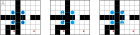
\includegraphics{sample1.pdf}
    \end{center}
    Läheme portaali 1 ja seejärel tõmbame kaks korda kangist, liikudes nii portaali 3.
    Samaaegselt liigub esimene münt, mis alguses asus samal ruudul portaaliga 4, portaali
    1 ja seejärel portaali 2. Nüüd saame minna ruutu $(3, 5)$, kus esimene münt
    nüüd asub, ja selle üles korjata. Seejärel läheme ruutu $(7, 7)$ ja korjame üles teise
    mündi. Kolmandat münti, mis asub ruudus $(7, 3)$, ei ole meil kunagi võimalik üles korjata,
    kuna ta on seintega ülejäänud ruudustikust eraldatud. Kokku korjasime üles kaks münti,
    mille koguväärtus on $2 + 3 = 5$.

    Teine näide on illustreeritud alljärgneval joonisel.
    \begin{center}
      
\includegraphics{sample2.pdf}
    \end{center}
    Selles näites on üksainus münt, mis asub esialgu samal ruudul portaaliga 4. Portaalide
    1 ja 2 vahel on võimalik käia, ülejäänud portaalid on ülejäänud ruudustikust eraldatud.
    Et münti kätte saada, läheme portaali 1 juurde ja tõmbame üheksa korda kangist.
    Meie asukoht muutub siis $1 \to 6 \to 7 \to 1 \to 6 \to 7 \to 1 \to 6 \to 7 \to 1$.
    Münt liigub samal ajal $4 \to 2 \to 5 \to 3 \to 4 \to 2 \to 5 \to 3 \to 4 \to 2$.
    Nüüd saame minna portaali 1 juurest portaali 2 juurde ja mündi üles korjata.
  \end{yl}
\end{ol}

\end{document}
